\documentclass[12pt,a4paper,oneside]{report}
\usepackage[margin=1in,headheight=15pt]{geometry}
\usepackage[T1]{fontenc}
\usepackage{lmodern}
\usepackage{microtype}
\usepackage{graphicx}
\usepackage{xcolor}
\usepackage{booktabs,tabularx,longtable,array}
\usepackage{amsmath,amssymb}
\usepackage{listings}
\usepackage{tikz}
\usetikzlibrary{arrows.meta,positioning,shapes.geometric}
\usepackage{hyperref}
\usepackage{fancyhdr}
\usepackage{caption}
\usepackage{enumitem}
\usepackage{float}
\definecolor{navy}{HTML}{142B4A}
\definecolor{blue}{HTML}{2463A6}
\definecolor{pale}{HTML}{EEF4FA}
\definecolor{codebg}{HTML}{F5F7FA}
\definecolor{green}{HTML}{247A58}
\hypersetup{colorlinks=true,linkcolor=blue,urlcolor=blue,citecolor=green,pdftitle={Algorithm Benchmarking and Profiling Suite},pdfauthor={IIT Dharwad Project Team}}
\pagestyle{fancy}\fancyhf{}\lhead{Algorithm Benchmarking and Profiling Suite}\rhead{Software Systems Lab}\cfoot{\thepage}
\lstset{basicstyle=\ttfamily\small,backgroundcolor=\color{codebg},frame=single,rulecolor=\color{black!15},breaklines=true,showstringspaces=false,columns=fullflexible,keywordstyle=\color{blue}\bfseries,commentstyle=\color{green!70!black},numbers=left,numberstyle=\tiny\color{black!45},xleftmargin=2em,framexleftmargin=1.5em}
\setlength{\parskip}{5pt}\setlength{\parindent}{0pt}
\begin{document}
\begin{titlepage}
\centering
\vspace*{1.0cm}
{\Large\bfseries INDIAN INSTITUTE OF TECHNOLOGY DHARWAD\par}
\vspace{0.25cm}{\large Software Systems Lab \;|\; CS202C\par}
\vspace{1.7cm}
{\color{blue}\rule{\linewidth}{1.5pt}}\\[0.5cm]
{\Huge\bfseries\color{navy} Algorithm Benchmarking\\[0.15cm] and Profiling Suite\par}
\vspace{0.45cm}{\Large Project Report\par}
\vspace{0.5cm}{\color{blue}\rule{\linewidth}{1.5pt}}
\vspace{1.3cm}
{\large\bfseries Submitted by\par}\vspace{0.35cm}
\begin{tabular}{ll}
Abhinav & CS25BT028\\
Jyoteen & CS25BT064\\
Shyam & CS25BT061\\
Gaurav & CS25BT024\\
Harsh & CS25BT019
\end{tabular}
\vfill
{\large\bfseries Faculty In-charge\par}\vspace{0.15cm}
{\Large Dr. Suman Dutta\par}
\vspace{0.8cm}{\large Academic Project Submission\par}
\vspace{0.4cm}{\large November 2026\par}
\end{titlepage}
\pagenumbering{roman}
\chapter*{Declaration}
We declare that this report describes the Algorithm Benchmarking and Profiling Suite developed by our team for the Software Systems Lab (CS202C). The implementation details are based on the submitted project source tree. The included Bubble Sort versus Merge Sort reference measurements were generated by executing the project's benchmark code in a Linux x86\_64 container during report preparation. They are identified as environment-specific reference measurements and are not represented as measurements from the team's own laptop.
\vspace{1cm}\textbf{Project team:} Abhinav, Jyoteen, Shyam, Gaurav and Harsh.\
\textbf{Institute:} Indian Institute of Technology Dharwad.
\chapter*{Acknowledgement}
We express our sincere gratitude to Dr. Suman Dutta for guidance and feedback during the Software Systems Lab project. We also acknowledge the open-source compiler, profiling and visualization tools used to build and evaluate the suite.
\chapter*{Abstract}
This project implements a command-line framework for comparing the execution time and profiling characteristics of two selected sorting algorithms on identical, reproducible integer datasets. The implementation combines C sorting routines with a shared C benchmark runner, Python-based dataset generation and repeated measurement, GNU Compiler Collection (GCC), GNU gprof, and GNUplot. Eleven sorting implementations are available: Bubble, Cocktail Shaker, Gnome, Insertion, Odd--Even Transposition, Selection, Heap, Merge, Quicksort, Radix and Shell sort. The workflow generates input sizes from 100 through 1000, compiles the selected implementations with consistent compiler flags, records the median of seven timing samples, performs profiling separately, and creates a log-scale runtime comparison plot. The report documents the architecture, implementation contract, algorithms, experimental controls, output artefacts, limitations and reproducibility procedure. A reference execution comparing Bubble Sort and Merge Sort is included with its timing table, graph, datasets, profiler reports and environment metadata. The report clearly distinguishes these reference measurements from results that would be obtained on the team's own evaluation machine.
\chapter*{Project at a Glance}
\begin{tabularx}{\textwidth}{>{\bfseries}p{0.29\textwidth}X}
Project & Algorithm Benchmarking and Profiling Suite\\
Course & Software Systems Lab (CS202C)\\
Institute & Indian Institute of Technology Dharwad\\
Faculty & Dr. Suman Dutta\\
Implementation & C, Python 3 and Bash\\
Build and profiling & GCC, GNU gprof\\
Visualization & GNUplot\\
Comparison model & Two sorting algorithms per execution\\
Dataset sizes & 100, 150, 200, \ldots, 1000 (19 sizes)\\
Timing statistic & Median of seven samples per algorithm and size\\
\end{tabularx}
\tableofcontents\listoffigures\listoftables\clearpage
\pagenumbering{arabic}
\chapter{Introduction}
\section{Background}
Algorithm analysis commonly begins with asymptotic complexity, but actual execution time is also affected by constant factors, memory access patterns, compiler settings, input characteristics and machine architecture. A practical benchmark helps connect theoretical expectations with observed behaviour. A profiler complements timing by indicating where a program spends its execution time.
\section{Problem Statement}
The project provides a repeatable way to select two sorting implementations, feed them the same generated data, measure their CPU time under a common harness, inspect profiling reports, and visualize how measured time changes with input size. Manual timing of separate programs is error-prone because inputs, compiler flags and measurement procedures may differ. The suite centralizes these steps.
\section{Objectives}
\begin{enumerate}[leftmargin=*]
\item Provide a menu-driven command-line selection of two distinct sorting source files.
\item Generate deterministic, non-negative integer datasets for a sequence of input sizes.
\item Use one common runner and consistent compilation settings for both algorithms.
\item Reduce timing noise by taking repeated samples and reporting their median.
\item Keep profiling runs separate from ordinary timing runs.
\item Store datasets, measurements, plots and profiler reports in a timestamped result directory.
\end{enumerate}
\section{Scope}
The current interactive workflow is a pairwise sorting benchmark. It offers eleven sorting implementations and compares two per run. Search and summation source files are also present in the wider algorithms directory, but they are not integrated into the current selection-and-comparison workflow. The report therefore does not describe them as supported benchmark modes.
\section{Expected Outcome}
A successful run produces a reproducible set of input files, a measurement data file, a runtime graph and two gprof reports. The benchmark is intended for comparative educational analysis, not as a universal ranking of algorithms across all hardware and workloads.

\chapter{System Overview and Architecture}
\section{High-Level Design}
The system is organized as a pipeline. The Bash script coordinates the workflow; Python generates datasets and aggregates timing samples; GCC builds the selected algorithm with the shared runner; gprof creates profiling reports; and GNUplot renders the runtime graph.
\begin{figure}[H]\centering
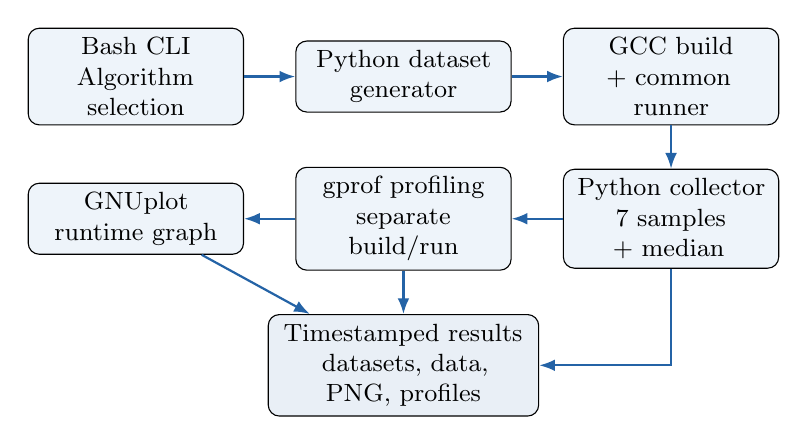
\begin{tikzpicture}[node distance=0.55cm and 0.65cm, every node/.style={draw,rounded corners,align=center,minimum height=0.85cm,text width=2.5cm,font=\small}, arr/.style={-{Latex[length=2mm]},thick,draw=blue}]
\node[fill=pale] (cli) {Bash CLI\\Algorithm selection};
\node[fill=pale,right=of cli] (data) {Python dataset\\generator};
\node[fill=pale,right=of data] (build) {GCC build\\+ common runner};
\node[fill=pale,below=of build] (measure) {Python collector\\7 samples + median};
\node[fill=pale,left=of measure] (profile) {gprof profiling\\separate build/run};
\node[fill=pale,left=of profile] (plot) {GNUplot\\runtime graph};
\node[fill=blue!10,below=of profile,text width=3.2cm] (out) {Timestamped results\\datasets, data, PNG, profiles};
\draw[arr] (cli)--(data);\draw[arr] (data)--(build);\draw[arr] (build)--(measure);\draw[arr] (measure)--(profile);\draw[arr] (profile)--(plot);\draw[arr] (measure)|-(out);\draw[arr] (profile)--(out);\draw[arr] (plot)--(out);
\end{tikzpicture}
\caption{End-to-end architecture of the implemented sorting benchmark.}\end{figure}
\section{Module Responsibilities}
\begin{longtable}{p{0.24\textwidth}p{0.68\textwidth}}
\toprule\textbf{Module} & \textbf{Responsibility}\\\midrule
\texttt{main/run.sh} & Validates dependencies, lists available C files, accepts two distinct choices, creates a unique run folder, compiles normal and profiling binaries, invokes collection, gprof and GNUplot.\\
\texttt{main/generate\_datasets.py} & Generates deterministic input files for each configured size using Python's seeded random number generator.\\
\texttt{algorithms/dataset/*.c} & Each selected source implements the common function contract and sorts a copy of the input into an output array.\\
\texttt{algorithms/dataset/runner.c} & Reads the input format, allocates arrays, repeats the algorithm call, measures CPU time using \texttt{clock()}, checks non-decreasing order and prints seconds per sort.\\
\texttt{main/collect.py} & Executes each normal binary seven times for every dataset, computes the median and writes the whitespace-separated measurement file.\\
\texttt{gprof} & Produces a separate profiling report from binaries compiled with \texttt{-pg}.\\
\texttt{gnuplot} & Produces a PNG line plot from the measurement file, using a logarithmic y-axis.\\
\bottomrule\end{longtable}
\section{Execution Flow}
\begin{enumerate}[leftmargin=*]
\item The user starts \texttt{main/run.sh}, optionally supplying two source paths; otherwise an interactive numbered list is shown.
\item The script validates required tools and checks that the selected files are distinct.
\item A timestamped directory is created under \texttt{results/}, with subdirectories for binaries, datasets and profiles.
\item The generator creates all 19 input datasets.
\item Each selected algorithm is compiled twice: a normal build and a profiling build.
\item The collector measures the normal binaries and writes the median timing table.
\item Profiling binaries are run on the size-1000 dataset, and gprof reports are saved.
\item GNUplot creates the runtime comparison PNG; the script prints the locations of all output artefacts.
\end{enumerate}

\chapter{Algorithm Implementations}
\section{Common Function Contract}
Each sorting source exports the same function:
\begin{lstlisting}[language=C]
void algorithm(const int *input, int *output, int n);
\end{lstlisting}
The input pointer is treated as read-only. Each implementation first copies the input values into the output buffer and sorts the output in place. This interface allows the same runner to benchmark different algorithms without changing its source code. It also ensures that every repeat starts from the original unsorted input rather than from the previous repeat's sorted output.
\section{Available Sorting Algorithms}
\begin{longtable}{p{0.22\textwidth}p{0.47\textwidth}p{0.22\textwidth}}
\toprule\textbf{Algorithm} & \textbf{Implementation idea} & \textbf{Typical time complexity}\\\midrule
Bubble sort & Repeatedly compare adjacent values and swap inversions; shrink the unsorted suffix. & $O(n^2)$\\
Cocktail Shaker sort & Bubble-sort passes in both left-to-right and right-to-left directions. & $O(n^2)$\\
Gnome sort & Move an out-of-order item backwards by adjacent swaps; advance when local order is correct. & $O(n^2)$\\
Insertion sort & Insert each next value into its correct position in the already-processed prefix. & $O(n^2)$ worst case\\
Odd--Even Transposition sort & Alternate comparisons of even-indexed and odd-indexed adjacent pairs until no swaps occur. & $O(n^2)$\\
Selection sort & Find the minimum remaining value and place it at the next output position. & $O(n^2)$\\
Heap sort & Build a max heap, then repeatedly move the maximum to the end and restore the heap. & $O(n\log n)$\\
Merge sort & Recursively split ranges, merge sorted halves using a scratch array. & $O(n\log n)$\\
Quicksort & Partition around a median-of-three pivot; recurse on the smaller side and iterate on the larger side. & Average $O(n\log n)$; worst $O(n^2)$\\
Radix sort & Perform four stable byte-wise counting passes over non-negative integer keys. & $O(4(n+256))$\\
Shell sort & Perform gapped insertion sorts using the Ciura gap sequence. & Gap-sequence dependent\\
\bottomrule\end{longtable}
\section{Implementation Notes}
The files labelled \texttt{unoptimized} provide elementary comparison-sort baselines. The files labelled \texttt{optimized} use alternative algorithmic strategies or implementation improvements; the labels are project naming conventions, not a claim that one implementation wins on every input. Merge sort and radix sort allocate temporary storage. Heap sort uses an iterative sift-down operation. Quicksort uses median-of-three pivot selection and smaller-partition recursion to limit recursion depth. Radix sort is explicitly designed for the non-negative integer values produced by the dataset generator.
\section{Complexity Interpretation}
Asymptotic complexity describes growth as input size increases; it does not directly predict a measured winner at the small sizes used here. For example, allocation overhead and cache behaviour can influence results. The experiment should therefore report observed measurements alongside, not instead of, theoretical complexity.

\chapter{Dataset Generation and Experimental Design}
\section{Dataset Construction}
The generator creates sizes from 100 to 1000 inclusive in increments of 50, resulting in 19 datasets. For a dataset of size $n$, it initializes a local pseudo-random generator with seed $2026+n$ and draws $n$ integers using \texttt{randrange(0, 1\_000\_000)}. Thus every generated value is in the interval $[0,999999]$. The file \texttt{n\_N.txt} contains the size on its first line and the values on the next line.
\begin{table}[H]\centering\caption{Dataset configuration}\begin{tabular}{ll}\toprule Parameter & Configured value\\\midrule First size & 100\\ Last size & 1000\\ Step & 50\\ Number of sizes & 19\\ Integer range & $0$ to $999999$ inclusive\\ Seed for size $n$ & $2026+n$\\ Dataset type & Pseudorandom, non-negative integers\\\bottomrule\end{tabular}\end{table}
Using the same saved dataset for both selected algorithms makes the comparison paired: both implementations receive identical values for a given $n$. Since the generator is deterministic for a fixed Python random implementation and seed, the data can be regenerated consistently in the same environment.
\section{Compilation Configuration}
The normal binaries are compiled with GCC using C11, debug information and warnings, with optimization disabled:
\begin{lstlisting}[language=bash]
gcc -std=c11 -O0 -g -Wall -Wextra -c algorithm.c -o algorithm.o
gcc -std=c11 -O0 -g -Wall -Wextra runner.c algorithm.o -o algorithm
\end{lstlisting}
The separate profiling build adds \texttt{-pg}. Using common flags for both normal builds helps reduce compiler-configuration differences. The \texttt{-O0} choice makes the implementation easier to inspect and keeps the compiler from optimizing away or substantially transforming the measured routines; it is not representative of a production-optimized build.
\section{Timing Procedure}
The collector performs seven independent process executions for every algorithm and dataset size. The C runner chooses a repeat count
\[
r=\max\left(10,\min\left(2000,\left\lfloor\frac{1,000,000}{n^2}\right\rfloor\right)\right).
\]
It reads the input once, then calls the algorithm $r$ times inside the timed region. CPU time is measured with the C standard library function \texttt{clock()}. The reported sample is
\[
t_{\mathrm{sample}}=\frac{(t_{\mathrm{stop}}-t_{\mathrm{start}})/\texttt{CLOCKS\_PER\_SEC}}{r}.
\]
The Python collector repeats the process seven times and records the median of those seven per-sort samples. Median is less sensitive than the mean to an unusually high or low sample. The plotted quantity is therefore median CPU seconds per sort, not wall-clock latency.
\section{Profiling Procedure}
The script compiles separate binaries with \texttt{-pg}. It runs each profiling binary on the size-1000 dataset for a default of 50 calls (overridable through \texttt{ABS\_PROFILE\_REPEATS}), then invokes \texttt{gprof -b}. The resulting text reports are stored separately under \texttt{profiles/}. Profiling instrumentation changes runtime, so these runs are intentionally excluded from the ordinary timing data and graph.
\section{Fairness and Controls}
\begin{itemize}[leftmargin=*]
\item Same generated data for both algorithms at each input size.
\item Separate output buffer and original input for every algorithm call.
\item Same C runner and normal compilation flags.
\item Seven process-level timing samples and median aggregation.
\item Profiling performed in a separate instrumented build.
\item A new timestamped output directory preserves each run's artefacts.
\end{itemize}

\chapter{Results, Outputs and Interpretation}
\section{Generated Artefacts}
A successful run creates a folder similar to \texttt{results/run\_YYYYMMDD\_HHMMSS/}. Its contents are:
\begin{longtable}{p{0.32\textwidth}p{0.58\textwidth}}
\toprule\textbf{Path} & \textbf{Purpose}\\\midrule
\texttt{datasets/n\_N.txt} & Exact input values used at each size.\\
\texttt{bin/} & Normal and profiling executables plus intermediate object files.\\
\texttt{benchmark\_data.dat} & Header and 19 rows containing $n$ and the median seconds per sort for each selected algorithm.\\
\texttt{runtime\_comparison.png} & GNUplot line graph with input size on x-axis and log-scaled median CPU time on y-axis.\\
\texttt{profiles/*\_gprof.txt} & gprof flat-profile reports for the two profiling binaries.\\
\bottomrule\end{longtable}
\section{How to Read the Runtime Graph}
The x-axis represents the number of input elements. The y-axis represents median CPU seconds per sort and is logarithmic, allowing curves with substantially different magnitudes to be visible together. A curve that rises more steeply as $n$ grows may indicate less favourable scaling over the tested range. A single crossing or small-size advantage should not be interpreted as a universal ranking.
\section{How to Read the Profiling Report}
The gprof flat profile lists functions and profiling statistics for the instrumented run. The algorithm function is the primary routine of interest, while helper functions may also appear depending on compiler and profiling behaviour. Profile percentages and times are specific to the selected size, repeat count, machine and build. They should be interpreted as diagnostic evidence, not as the same measurement used in the runtime graph.
\section{Measured Benchmark: Bubble Sort vs.\ Merge Sort}
To provide a concrete end-to-end example, the project workflow was executed during preparation of this report using the repository's own dataset generator, C runner and active Python collector. The selected comparison is \texttt{bubble\_unoptimized.c} against \texttt{merge\_optimized.c}. Both algorithms were compiled with the same normal-build flags and received the exact same 19 deterministic datasets.

\begin{figure}[H]
\centering
\includegraphics[width=0.94\textwidth]{../results/reference_run_20261111/runtime_comparison.png}
\caption{Measured median CPU time per sort for Bubble Sort and Merge Sort. The vertical axis is logarithmic.}
\label{fig:runtime-comparison}
\end{figure}

\begin{table}[H]\centering
\caption{Selected measured points from the benchmark data file}
\begin{tabular}{rrrr}
\toprule
\textbf{Input size} & \textbf{Bubble sort (s)} & \textbf{Merge sort (s)} & \textbf{Bubble/Merge ratio}\\
\midrule
100 & $1.1450\times10^{-5}$ & $3.1800\times10^{-6}$ & 3.60$\times$\\
500 & $3.1520\times10^{-4}$ & $3.1200\times10^{-5}$ & 10.10$\times$\\
1000 & $1.3332\times10^{-3}$ & $7.0700\times10^{-5}$ & 18.86$\times$\\
\bottomrule
\end{tabular}
\end{table}

\subsection{Discussion}
Across this reference run, Bubble Sort's median time rises from approximately $11.45$ microseconds at $n=100$ to $1.333$ milliseconds at $n=1000$. Merge Sort rises from approximately $3.18$ microseconds to $70.7$ microseconds over the same range. At the largest tested size, Merge Sort is approximately 18.9 times faster in this particular run. The widening gap is consistent with the expected growth difference between a quadratic comparison sort, $O(n^2)$, and a divide-and-conquer sort, $O(n\log n)$.

This is an observed result for the selected pair, generated data, compiler settings and execution environment; it is not a universal ranking of all eleven algorithms. The small input range, unoptimized \texttt{-O0} build, timer resolution and host load can affect the values. The full 19-row dataset is included at \texttt{results/reference\_run\_20261111/benchmark\_data.dat}.

\subsection{Profiling observations}
The two profiling binaries were built separately with \texttt{-pg} and run on the size-1000 dataset for 50 calls, matching the workflow's default. gprof attributed measurable sampled time to Bubble Sort's \texttt{algorithm} function. For Merge Sort, the short profiling run was too brief for gprof's sampling resolution to accumulate a meaningful time value, although its call graph recorded calls to \texttt{algorithm}, \texttt{merge\_sort} and \texttt{merge}. This illustrates why profiler output must be interpreted with its sampling resolution and workload duration in mind. The profiling reports are preserved in the results folder.

\subsection{Execution environment and reproducibility}
The reference measurements were generated on a Linux x86\_64 container with GCC 14.2.0, Python 3.13.5 and three logical CPUs exposed to the container. All eleven sorting source files were also compiled and linked successfully against the shared runner as a source-tree build check. Since GNUplot was not installed in this report-preparation container, the included graph was rendered with Matplotlib from the exact measured \texttt{benchmark\_data.dat} values; the project's normal \texttt{main/run.sh} still uses GNUplot. Both algorithms used \texttt{-std=c11 -O0 -g -Wall -Wextra}; the separate profiling build added \texttt{-pg}. Each of the 19 input sizes used seven process-level samples, with the median reported. Dataset generation used seed $2026+n$ and values in $[0,999999]$.

\textbf{Important:} these are actual measurements from the execution environment used to prepare this report, not measurements from the team's laptop or evaluation machine. Re-run \texttt{main/run.sh} on the target machine to obtain its machine-specific measurements. The included \texttt{environment.json}, datasets, timing table, graph and gprof reports make this reference run inspectable and reproducible.

\chapter{How to Build and Run}
\section{Prerequisites}
The workflow is designed for Linux or Windows Subsystem for Linux (WSL) and requires Python 3, GCC, GNU gprof, GNUplot and NumPy. The WSL environment must have a Linux distribution installed and virtualization enabled. Install missing Ubuntu packages with:
\begin{lstlisting}[language=bash]
sudo apt update
sudo apt install build-essential binutils gnuplot python3 python3-numpy
\end{lstlisting}
\section{Run Commands}
From the project root:
\begin{lstlisting}[language=bash]
chmod +x main/run.sh
./main/run.sh
\end{lstlisting}
Choose two different algorithm numbers when prompted. The script also accepts two source paths directly:
\begin{lstlisting}[language=bash]
./main/run.sh algorithms/dataset/bubble_unoptimized.c \\
  algorithms/dataset/merge_optimized.c
\end{lstlisting}
For help:
\begin{lstlisting}[language=bash]
./main/run.sh --help
\end{lstlisting}
To change the number of calls in the separate profiling run:
\begin{lstlisting}[language=bash]
ABS_PROFILE_REPEATS=100 ./main/run.sh
\end{lstlisting}
\section{Troubleshooting}
If a required command is missing, install the corresponding package and rerun. If WSL reports that virtualization is disabled, enable CPU virtualization in firmware settings and ensure the Windows Virtual Machine Platform feature is enabled, then restart. If GNUplot cannot create a PNG, verify that GNUplot is installed and available on \texttt{PATH}. If a selected algorithm fails to compile, inspect compiler diagnostics; all sorting implementations must provide the exact common function signature.

\chapter{Testing, Validation and Limitations}
\section{Implemented Checks}
The runner validates the input header and repeat count, checks allocation and input-read failures, checks that the clock calls succeed, and verifies that the final output is in non-decreasing order. The generator validates positive size parameters. The shell script checks required tools, support files, distinct source selections, compilation success, profiling output and plot creation. The collector checks for missing dataset files and rejects failed subprocess executions or invalid timing output.
\section{Important Validation Limitation}
The runner currently checks sorted order only. It does not compare the output against a sorted reference or verify that the output contains exactly the same multiset of elements as the input. A routine that accidentally drops or changes values could theoretically pass the order check. A stronger future validation should compare output against a trusted reference sort or check both sortedness and element preservation before accepting a timing sample.
\section{Other Limitations}
\begin{itemize}[leftmargin=*]
\item Only two sorting algorithms are compared in each run; a full all-pairs or all-algorithms campaign requires repeated runs.
\item The generated workload is one random, non-negative integer distribution. Sorted, reverse-sorted, duplicate-heavy and nearly sorted datasets are not currently generated by this workflow.
\item The tested input sizes stop at 1000, which may be too small to reveal asymptotic behaviour clearly for some algorithms.
\item CPU time from \texttt{clock()} is not wall-clock response time and can be affected by platform timer resolution.
\item The compiler uses \texttt{-O0}; results may differ under optimized release builds.
\item Radix sort assumes non-negative integer keys, matching the generator's range.
\item gprof sampling/instrumentation has overhead and its reports are not directly comparable to uninstrumented timing values.
\end{itemize}
\section{Future Improvements}
Add permutation-preserving correctness checks; support multiple dataset distributions; increase and configure input-size ranges; export CSV with explicit units and environment metadata; automate all-algorithm comparisons; add wall-clock timing alongside CPU time; compare debug and optimized compiler builds; and add automated unit tests for each sorting implementation.

\chapter{Conclusion}
The Algorithm Benchmarking and Profiling Suite provides an integrated, repeatable workflow for comparing two selected C sorting algorithms. It combines deterministic dataset generation, a shared runner, repeated median-based CPU-time measurement, separate gprof profiling and GNUplot visualization. The available implementations cover six elementary quadratic sorts and five alternative sorting strategies. The project demonstrates how algorithmic ideas can be evaluated through controlled experiments while preserving the distinction between theoretical complexity, measured runtime and profiler output. The next step for a complete experimental study is to execute the workflow on the target machine, retain its generated artefacts and add conclusions based only on those observations.

\appendix
\chapter{Source Tree Reference}
\begin{lstlisting}
Algorithm-Benchmark/
|-- algorithms/dataset/
|   |-- bubble_unoptimized.c
|   |-- cocktail_unoptimized.c
|   |-- gnome_unoptimized.c
|   |-- insertion_unoptimized.c
|   |-- odd_even_unoptimized.c
|   |-- selection_unoptimized.c
|   |-- heap_optimized.c
|   |-- merge_optimized.c
|   |-- quicksort_optimized.c
|   |-- radix_optimized.c
|   |-- shell_optimized.c
|   `-- runner.c
|-- main/
|   |-- generate_datasets.py
|   |-- collect.py
|   `-- run.sh
|-- docs/
|-- report/
`-- presentation/
\end{lstlisting}
The root-level `collect.py` is a legacy standalone collector and is not invoked by `main/run.sh`; the active collection step is `main/collect.py`.
\chapter{Team Details}
\begin{table}[H]\centering\begin{tabular}{ll}\toprule Name & Roll number\\\midrule Abhinav & CS25BT028\\ Jyoteen & CS25BT064\\ Shyam & CS25BT061\\ Gaurav & CS25BT024\\ Harsh & CS25BT019\\\bottomrule\end{tabular}\end{table}
\textbf{Course:} Software Systems Lab (CS202C)\\\textbf{Faculty:} Dr. Suman Dutta\\\textbf{Institute:} Indian Institute of Technology Dharwad.
\begin{thebibliography}{9}
\bibitem{cstandard} ISO/IEC 9899, Programming Languages --- C.
\bibitem{gcc} GNU Project, \emph{GCC Documentation}, \url{https://gcc.gnu.org/onlinedocs/}.
\bibitem{gprof} GNU Project, \emph{GNU gprof Documentation}, \url{https://sourceware.org/binutils/docs/gprof/}.
\bibitem{gnuplot} GNUplot Development Team, \emph{GNUplot Documentation}, \url{http://www.gnuplot.info/documentation.html}.
\bibitem{python} Python Software Foundation, \emph{Python 3 Documentation}, \url{https://docs.python.org/3/}.
\end{thebibliography}
\end{document}
